\chapter{Related work}\label{ch:related} % 6

Work on deterministic parallel programming models is long-standing.
As we have seen, what deterministic parallel programming models have
in common is that they all must do something to restrict access to
mutable state shared among concurrent computations so that schedule
nondeterminism cannot be observed.  Depending on the model,
restricting access to shared mutable state might involve disallowing
sharing entirely~\cite{dph}, only allowing single assignments to
shared references~\cite{Tesler-1968, IStructures, CnC}, allowing
sharing only by a limited form of message passing~\cite{Kahn-1974},
ensuring that concurrent accesses to shared state are
disjoint~\cite{dpj-oopsla}, resolving conflicting updates after the
fact~\cite{concurrent-revisions-haskell11}, or some combination of
these approaches.  These constraints can be imposed at the language or
API level, within a type system or at runtime.

In particular, the LVars model was inspired by two traditional
deterministic parallel programming models based on
monotonically-growing shared data structures: first, Kahn process
networks~\cite{Kahn-1974}, in which a network of processes communicate
with each other through blocking FIFO channels with ever-growing
{\emph channel histories}; and, second, IVars~\cite{IStructures},
single-assignment locations with blocking read semantics.

LVars are general enough to subsume both IVars and KPNs: a lattice of
channel histories with a prefix ordering allows LVars to represent
FIFO channels that implement a Kahn process network, whereas
instantiating $\lambdaLVar$ with a lattice with one ``empty'' state
and multiple ``full'' states (where $\forall{i}.\; \mathit{empty} <
\mathit{full_i}$) results in a parallel single-assignment language
with a store of IVars, as we saw in \either{Chapter}{Section}~\ref{ch:lvars}.  Hence
LVars provide a framework for generalizing and unifying these two
existing approaches to deterministic parallelism.  In this \either{chapter}{section}, \either{I}{we}
describe some more recent contributions to the literature, and how the
LVars model relates to them.

\section{Deterministic Parallel Java (DPJ)}

DPJ \cite{dpj-oopsla, dpj-hotpar09} is a deterministic language
consisting of a system of annotations for Java code.  A sophisticated
region-based type system ensures that a mutable region of the heap is,
essentially, passed linearly to an exclusive writer, thereby ensuring
that the state accessed by concurrent threads is disjoint.  DPJ does,
however, provide a way to unsafely assert that operations commute with
one another (using the @commuteswith@ form) to enable concurrent
mutation.

The LVars model differs from DPJ in that it allows overlapping shared
state between threads as the default.  Moreover, since LVar effects
are already commutative, we avoid the need for @commuteswith@
annotations.  Finally, it is worth noting that while in DPJ,
commutativity annotations have to appear in application-level code, in
LVish only the data-structure author needs to write trusted code. The
application programmer can run untrusted code that still enjoys a
(quasi-)determinism guarantee, because only (quasi-)deterministic
programs can be expressed as LVish @Par@ computations.
More recently, Bocchino \etal~\shortcite{dpj-popl} proposed a type and
effect system that allows for the incorporation of nondeterministic
sections of code in DPJ.  The goal here is different from ours: while
they aim to support \emph{intentionally} nondeterministic computations
such as those arising from optimization problems like branch-and-bound
search, the quasi-determinism in LVish arises as a result of schedule
nondeterminism.

\section{FlowPools}

Prokopec \etal~\shortcite{flowpools} propose a data structure with an API
closely related to LVars extended with freezing and handlers: a
FlowPool is a bag (that is, a multiset) that allows concurrent
insertions but forbids removals, a @seal@ operation that forbids
further updates, and combinators like @foreach@ that invoke callbacks
as data arrives in the pool.  To retain determinism, the @seal@
operation requires explicitly passing the expected bag \emph{size} as
an argument, and the program will raise an exception if the bag goes
over the expected size.

While this interface has a flavor similar to that of LVars, it lacks
the ability to detect quiescence, which is crucial for expressing
algorithms like graph traversal, and the @seal@ operation is awkward
to use when the structure of data is not known in advance.  By
contrast, the @freeze@ operation on LVars does not require such
advance knowledge, but moves the model into the realm of
quasi-determinism.  Another important difference is the fact that
LVars are \emph{data structure-generic}: both our formalism and our
library support an unlimited collection of data structures, whereas
FlowPools are specialized to bags.

\section{Concurrent Revisions}

Burckhardt \etal~\shortcite{eventually-consistent-transactions}
propose a formalism for eventual consistency based on graphs called
\emph{revision diagrams}, and Leijen, Burckhardt, and Fahndrich apply
the revision diagrams approach to guaranteed-deterministic concurrent
functional programming~\shortcite{concurrent-revisions-haskell11}.
Their \emph{Concurrent Revisions} (CR) programming model uses
isolation types to distinguish regions of the heap shared by multiple
mutators.  Rather than enforcing exclusive access in the style of DPJ,
CR clones a copy of the state for each mutator, using a deterministic
``merge function'' for resolving conflicts in local copies at join
points.

\ifdefined\DISSERTATION
\begin{wrapfigure}{r}{3in}
\vspace{-1em}
\begin{center}
  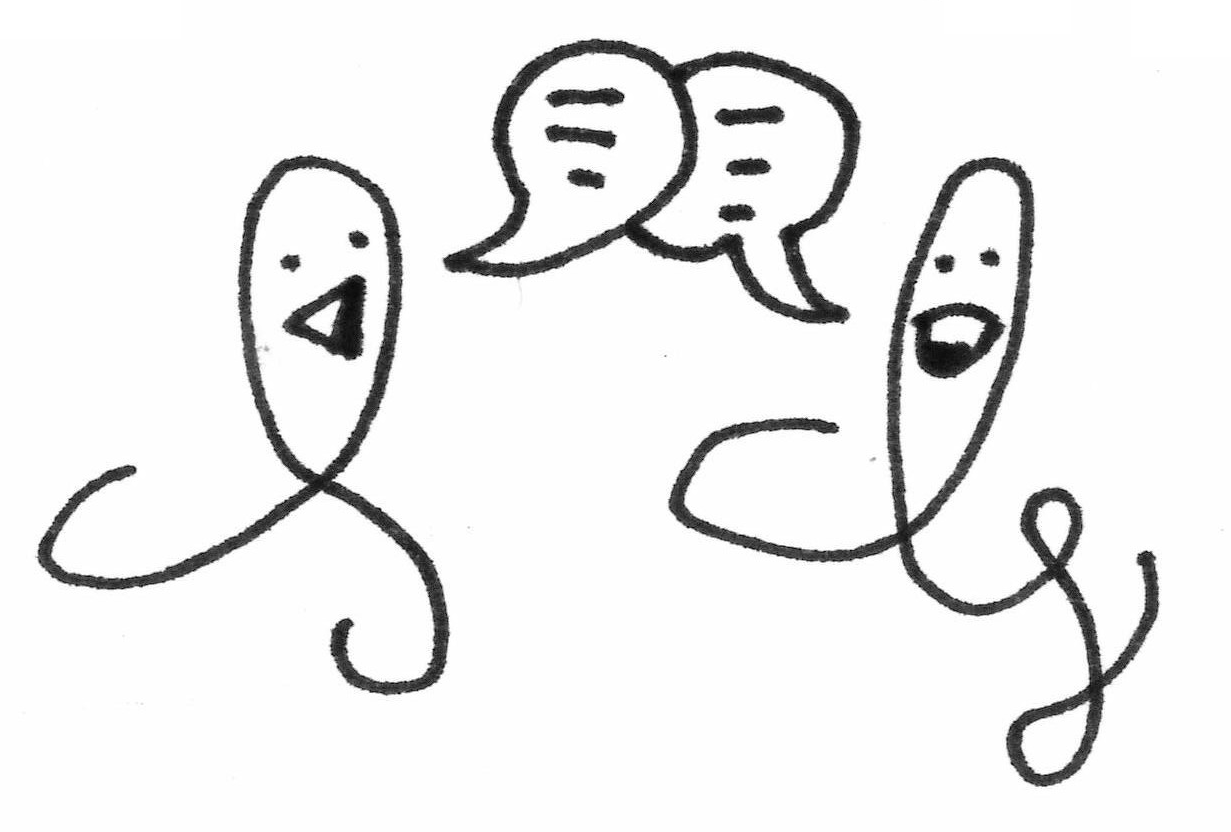
\includegraphics[scale=0.15]{../illustrations/communicating-threads}
\end{center}
\vspace{-2em}
\end{wrapfigure}
\fi

In CR, variables can be annotated as being shared between a ``joiner''
thread and a ``joinee'' thread.  Unlike the lub writes of LVars, CR
merge functions are \emph{not} necessarily commutative; indeed, the
default CR merge function is ``joiner wins''.  Determinism is enforced
by the programming model allowing the programmer to specify which of
two writing threads should prevail, regardless of the order in which
those writes arrive, and the states that a shared variable can take on
need not form a lattice.  Still, semilattices turn up in the
metatheory of CR: in particular, Burckhardt and
Leijen~\shortcite{semantics-concurrent-revisions} show that revision
diagrams are semilattices, and that therefore, for any two vertices in
a CR revision diagram, there exists a \emph{greatest common ancestor}
state that can be used to determine what changes each side has
made---an interesting duality with the LVars model (in which any two
LVar states have a lub).

Although versioned variables in CR could model lattice-based data
structures---if they used the lub operation as their merge function
for conflicts---the programming model nevertheless differs from the
LVars model in that effects only become visible at the end of parallel
regions, as opposed to the asynchronous communication within parallel
regions that the LVars model allows.  This semantics precludes the use
of traditional lock-free data structures for representing versioned
variables.

\section{Conflict-free replicated data types}
\ifdefined\JOURNAL

Shapiro~\etal's \emph{conflict-free replicated data types}
(CRDTs)~\shortcite{crdts,crdts-tr} provide a simple mathematical framework
for reasoning about and enforcing the \emph{eventual consistency} of
replicated objects in a distributed system.  Lattice-based CRDTs,
known as \emph{convergent replicated data types} or CvRDTs, view
replica states as elements of a lattice and replica conflict
resolution as the lattice's join operation.  As with LVars, the
contents of a CvRDT data structure can only grow with respect to the
given lattice.  Although LVars and CvRDTs were developed
independently, both models leverage the mathematical properties of
join-semilattices to ensure that a property of the model
holds---determinism in the case of LVars; eventual consistency in the
case of CvRDTs.  However, with CvRDTs (unlike with LVars), it is
possible to observe inconsistent \emph{intermediate} states of
replicated shared objects, and high availability requires that reads
return a value immediately, even if that value is stale.  Our work on
equipping CvRDTs with LVar-style threshold reads (which would allow
for deterministic reads at the price of high availability) is
ongoing~\cite{joining-wodet, lvars-dissertation}.  \fi

\ifdefined\DISSSERTATION
In Chapter~\ref{ch:distributed}, I presented a way to equip
lattice-based distributed data structures with LVar-style threshold
reads, resulting in a way to make deterministic \emph{threshold
  queries} of them.  My approach is based on Shapiro \etal's work on
conflict-free replicated data types (CRDTs) \cite{crdts,crdts-tr} and
in particular their work on the lattice-based formulation of CRDTs,
called \emph{convergent replicated data types} or CvRDTs, which I
discuss in detail in Section~\ref{s:distributed-cvrdts}.

As we saw in Chapter~\ref{ch:distributed}, database services such as
Amazon's SimpleDB~\cite{simpledb-vogels-article} allow for both
eventually consistent and strongly consistent reads, chosen at a
per-query granularity.  Terry~\etal's Pileus key-value
store~\cite{pileus} takes the idea of mixing consistency levels
further: instead of requiring the application developer to choose the
consistency level of a particular query at development time, the
system allows the developer to specify a service-level agreement that
can dynamically adapt to changing network conditions, for instance.
Hence choosing consistency at a per-query level and mixing consistency
levels within a single application is not a new idea.  Rather, the new
contribution that I make by adding threshold queries to CvRDTs is to
establish lattice-based data structures as a unifying formal
foundation for both eventually consistent and strongly consistent
queries.
\fi

\section{Bloom and Bloom$^L$}

Other authors have also used lattices as a framework for establishing
formal guarantees about eventually consistent systems and distributed
programs.  The Bloom language for distributed database programming
guarantees eventual consistency for distributed data collections that
are updated monotonically.  The initial formulation of
Bloom~\cite{bloom-cidr} had a notion of monotonicity based on set
inclusion, which is analogous to the store ordering relation in the
(IVar-based) Featherweight CnC system that \either{I}{we} described in
Section~\ref{subsection:lvars-monotonic-store-growth}.  Later, Conway
\etal~\shortcite{blooml} generalized Bloom to a more flexible
lattice-parameterized system, Bloom$^L$, in a manner analogous to the
generalization from IVars to LVars.  Bloom$^L$ combines ideas from the
aforementioned work on CRDTs~\cite{crdts, crdts-tr} with
\emph{monotonic logic}, resulting in a lattice-parameterized,
confluent language that is a close (but independently invented)
relative to the LVars model.  Bloom($^L$) is implemented as a
domain-specific language embedded in Ruby, and a monotonicity analysis
pass rules out programs that would perform non-monotonic operations on
distributed data collections (such as the removal of elements from a
set).  By contrast, in the LVars model (and in the LVish library),
monotonicity is enforced by the API presented by LVars, and since the
LVish library is implemented in Haskell, we can rely on Haskell's type
system for fine-grained effect tracking and monadic encapsulation of
LVar effects.

\section{Frame properties and separation logics}\label{s:related-frame-properties-and-separation-logics}

In Section~\ref{subsection:lvars-independence}, we saw that the
Independence lemma, Lemma~\ref{lem:lvars-independence}, expresses a
\emph{frame property} reminiscent of the following \emph{frame rule}
from separation logic and concurrent separation
logic~\cite{OHearnLocalReasoning, ReynoldsSeparationLogic,
  OHearnResourcesConcurrency}:
\begin{mathpar}
  \inferrule*
      {\lbrace p \rbrace ~ C ~ \lbrace q \rbrace}
      {\lbrace p * r \rbrace ~ C ~ \lbrace q * r \rbrace}
\end{mathpar}
Recall that the separating conjunction connective $*$ says that the
assertions it combines can be satisfied in a non-overlapping manner;
for instance, $p * r$ is satisfied by a heap if the heap can be split
into two non-overlapping parts satisfying $p$ and $r$, respectively.
However, sometimes we do in fact want to allow some amount of
``physical'' overlap between resources, while retaining ``logical'' or
``fictional'' separation.  In fact, the Independence lemma, since it
replaces the separating conjunction with the lub operation, allows
overlap between the original store and the ``frame'' store $S''$;
indeed, the point of LVars is that total disjointness is unnecessary,
since updates commute.  Jensen and Birkedal's recent work on
\emph{fictional separation logic}~\shortcite{JensenBirkedalFictional}
explores the notion of fictional separation in detail, generalizing
traditional separation logic to allow much more sophisticated kinds of
sharing.

Even more recently, Dinsdale-Young \etal~\shortcite{views} introduced the
``Views'' framework, which brings the notion of fictional separation
to a concurrent setting.  The Views framework is a metatheory of
concurrent reasoning principles that generalizes a variety of
concurrent program logics and type systems, including concurrent
separation logic.  It provides a generalized frame rule, which is
parameterized by a function $f$ that is applied to the pre- and
post-conditions in the conclusion of the rule:
\begin{mathpar}
  \inferrule*
      {\lbrace p \rbrace ~ C ~ \lbrace q \rbrace}
      {\lbrace f(p) \rbrace ~ C ~ \lbrace f(q) \rbrace}
\end{mathpar}
In this formulation of the rule, the ``frame'' is an abstract piece of
knowledge that is not violated by the execution of $C$.  The
Generalized Independence lemma
(Lemma~\ref{lem:generalized-independence}) that \either{I}{we} describe in
Section~\ref{subsection:quasi-generalized-independence}, which extends
the Independence lemma to handle arbitrary update operations, is
reminiscent of this generalized frame rule.
